% !TEX TS-program = lualatex+se
% !TEX encoding = UTF-8

\documentclass[oneside, 12pt, a4paper]{book}
\usepackage[letterpaper,showframe]{geometry}
\usepackage{fullpage} % redukcja marginesów
\usepackage{geometry}
\geometry{
	left=15mm,
	right=10mm,
	top=12mm,
	bottom=12mm,
	marginparwidth=0mm,
	marginparsep=0mm
	}
\usepackage{gregoriotex}
\gresetlinecolor{gregoriocolor}
\gresetheadercapture{annotation}{greannotation}{string}
% Format annotation above initial
\grechangestyle{annotation}{\small\bfseries}%
\grechangedim{intersyllablespacenotes}{0.18cm}{scalable}%

\usepackage{fullpage}
\usepackage{multicol}

%  Konfiguracja kolumn
\usepackage{paracol}
\setcolumnwidth{13.6cm,4cm}
\setlength{\columnsep}{0.4cm}
% \setlength{\columnseprule}{0.4pt}
% \colseprulecolor{red}

\usepackage{Tabbing}
\usepackage{longtable}
\usepackage[savepos]{zref}

\let\grelocalleftbox\localleftbox
\let\grelocalrightbox\localrightbox

\usepackage[latin,polish]{babel}

\usepackage{fontspec}
\defaultfontfeatures{Ligatures=TeX}
\setmainfont{Libertinus Serif}

\pagestyle{empty}	% usuwanie nagłówków/stopek z dokumentu
\usepackage[indent=0pt]{parskip} % ustawianie paragrafów
%\usepackage{setspace} % odstępy między liniami
%\setstretch{1.5} % półtorej linii odległości między wierszami

\usepackage{graphicx} % umożliwia import obrazów
\graphicspath{{img/}} % katalog obrazów

\usepackage{titlesec} % ustawianie nagłówków
\titlespacing*{\chapter}{0pt}{0pt}{0pt}	
\titleformat{\chapter}[hang]{\filcenter\large\scshape\bfseries}{}{0pt}{} % format nagłówków

\newfontface\vectis{VectisMonumentalW01-Regular}
\def\greinitialformat#1{\fontsize{20}{20}\vectis #1}

\begin{document}
\newcommand{\red}[1]{\textcolor{red}{#1}}
\newcommand{\black}[1]{\textcolor{black}{#1}}
\setlength{\parindent}{0pt}
\gresetbracerendering{font}

\pagenumbering{gobble} % nie jest wyprowadzany żaden numer strony, chociaż numer jest nadal resetowany. Odniesienia do tej strony również są puste.

%% ----------------- STRONA TYTUŁOWA  ---------------------
\begin{center}
	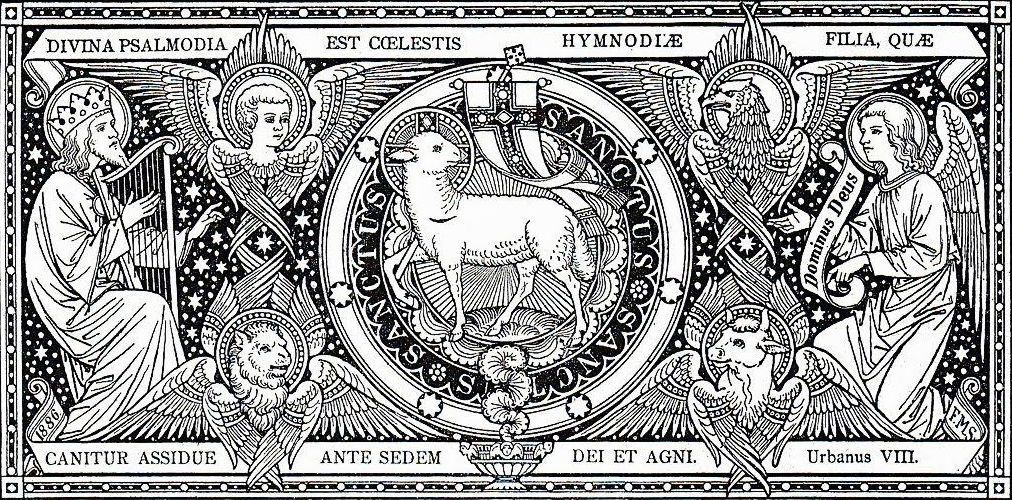
\includegraphics[width=1.0\textwidth]{divina_psalmodia.jpg}
	\vfill
	\fontspec{jsl-ancient.ttf}
	\fontsize{36}{40}\selectfont
	\textbf{Hymny laudesowe}\par
	\normalfont
	\vfill
	
\includegraphics[width=0.6\textwidth]{benedicamus_domino.jpg}
\end{center}

%% -----------------  SPIS TREŚCI ---------------------
\tableofcontents
\pagenumbering{arabic}
%% -----------------  HYMNY Commune Confessoris Pontificis ---------------------
\chapter{Jesu Redemptor omnium (Commune Confessoris Pontificis)}
\begin{center}
	\noindent\textit{Liber antiphonarius, 1960, p. 57}
\end{center}	
\vspace{5mm}
\begin{paracol}{2}
	\ensurevspace{5cm}
	{\greannotation{Hymn.}\greannotation{4} \gabcsnippet{(c4)Je(gh)su(g) Re(hi)dém(i)ptor(hg) óm(h')ni(h)um,(i.) (,) Per(j)pes(h') co(h)ró(h)na(h) Prǽ(i')su(g)lum,(g.) (;) In(g) hac(i') di(g)e(h) cle(g)mén(ef)ti(e)us(d.) (,) In(g)dúl(hi)ge(g)as(h) pre(g)cán(hiwj)ti(h)bus.(i.) (::) }}
	\switchcolumn
	{\parbox[c]{4cm}{Jezu, Odkupicielu wszystkich, Wiekuista korono Biskupów, W dniu dzisiejszym łaskawiej Wybacz proszącym.}}
  	\ensurevspace{5cm}
	\switchcolumn*
	{\gresetinitiallines{0}\gabcsnippet{2. Tu(gh)i(g) sa(hi)cri(i) qua(hg) nó(h')mi(h)nis(i.) (,) Con(j)fés(h')sor(h) al(h)mus(h) clá(i')ru(g)it:(g.) (;) Hu(g)jus(i') ce(g)lé(h)brat(g) án(ef)nu(e)a(d.) (,) De(g)vó(hi)ta(g) plebs(h) so(g)lém(hiwj)ni(h)a.(i.) (::) }}
	\switchcolumn
	{\parbox[c]{4cm}{Którego to dnia zajaśniał Błogosławiony Wyznawca twego imienia: Tegoż doroczną uroczystość Obchodzi lud wierny.}}
	\ensurevspace{5cm}
	\switchcolumn*
	{\gresetinitiallines{0}\gabcsnippet{3. Qui(gh) ri(g)te(hi) mun(i)di(hg) gáu(h')di(h)a(i.) (,) Hu(j)jus(h') ca(h)dú(h)ca(h) ré(i')spu(g)ens,(g.) (;) Æ(g)ter(i')ni(g)tá(h)tis(g) prǽ(ef)mi(e)o(d.) (,) Po(g)tí(hi)tur(g) in(h)ter(g) Án(hiwj)ge(h)los.(i.) (::) }}
	\switchcolumn
	{\parbox[c]{4cm}{Gardząc słusznie znikomemi Radościami tego świata, Posiadł nagrodę wiecznościMiędzy Aniołami.}}
	\ensurevspace{5cm}
	\switchcolumn*
	{\gresetinitiallines{0}\gabcsnippet{4. Hu(gh)jus(g) be(hi)ní(i)gnus(hg) án(h')nu(h)e(i.) (,) No(j)bis(h') se(h)qui(h) ve(h)stí(i')gi(g)a:(g.) (;) Hu(g)ius(i') pre(g)cá(h)tu,(g) sér(ef)vu(e)lis(d.) (,) Di(g)mít(hi)te(g) no(h)xam(g) crí(hiwj)mi(h)nis.(i.) (::)}}
	\switchcolumn
	{\parbox[c]{4cm}{Dozwól nam dobrotliwie Chodzić jego śladami; Na jego prośbę odpuść Sługom winę grzechu.}}
	\ensurevspace{5cm}
	\switchcolumn*
	{\gresetinitiallines{0}\gabcsnippet{5. Sit(gh) Chri(g)ste,(hi) Rex(i) pi(hg)ís(h')si(h)me,(i.) (,) Ti(j)bi,(h') Pa(h)trí(h)que(h) gló(i')ri(g)a,(g.) (;) Cum(g) Spí(i')ri(g)tu(h) Pa(g)rá(ef)cli(e)to,(d.) (,) Nunc,(g) et(hi) per(g) om(h)ne(g) sǽ(hiwj)cu(h)lum.(i.) (::) A(iji)men.(hi..) (::)}}
	\switchcolumn
	{\parbox[c]{4cm}{Tobie, Chryste, Królu najmiłościwszy, I Ojcu niechaj będzie chwała Wespół z Duchem Pocieszycielem Teraz i po wszystek wiek. Amen.}}
\end{paracol}	
%% -----------------  HYMNY Commune Confessoris non Pontificis---------------------
\chapter{Iste Confessor (Commune Confessoris non Pontificis)}
\begin{center}
	\textit{Liber Usualis, 1961, p. 1196}
\end{center}	
\vspace{5mm}
\begin{paracol}{2}
	\ensurevspace{5cm}
	{\greannotation{Hymn.} \gabcsnippet{(f3) I(f)ste(e) Con(fh)fés(hg)sor(fg) Dó(f')mi(f)ni,(e') co(f)lén(h)tes(h.) (;) Quem(ih) pi(i)e(j) lau(ih)dant(i.) (,) pó(h')pu(g)li(f') per(g) or(f)bem,(e.) (:) Hac(hhg) di(f')e(e) lae(h)tus(h.) (,) mé(i')ru(j)it(i') su(h)pré(g)mos(f.) (,) Lau(h)dis(g') ho(h)nó(fe)res.(f.) (::) }}
	\switchcolumn
	{\parbox[c]{4cm}{Oto wyznawca Pański, Którego pobożnie czcząc, wysławiają ludy po świecie, Dziś zasłużył radośnie, na najwyższe zaszczyty chwały.}}
  	\ensurevspace{5cm}
	\switchcolumn*
	{\gresetinitiallines{0}\gabcsnippet{2. Qui(f) pi(e)us,(fh) pru(hg)dens,(fg) hú(f')mi(f)lis,(e') pu(f)dí(h)cus,(h.) (;) Só(ih)bri(i)am(j) du(ih)xit(i.) (,) si(h')ne(g) la(f')be(g) vi(f)tam,(e.) (:) Do(hhg)nec(f') hu(e)má(h)nos(h.) (,) a(i')ni(j)má(i')vit(h) au(g)rae(f.) (,) Spí(h)ri(g')tus(h) ar(fe)tus.(f.) (::) }}
	\switchcolumn
	{\parbox[c]{4cm}{Bogobojny, mądry, pokorny, wstydliwy, wiódł życie wstrzemięźliwe, bez zmazy, dopóki tchnienie ducha ożywiało członki człowiecze.}}
	\ensurevspace{5cm}
	\switchcolumn*
	{\gresetinitiallines{0}\gabcsnippet{3. Cu(f)jus(e) ob(fh) prae(hg)stans(fg) mé(f')ri(f)tum(e') fre(f)quén(h)ter,(h.) (;) Ae(ih)gra(i) quae(j) pas(ih)sim(i.) (,) ja(h')cu(g)é(f')re(g) mem(f)bra,(e.) (:) Ví(hhg)ri(f')bus(e) mor(h)bi(h.) (,) dó(i')mi(j)tis,(i') sa(h)lú(g)ti(f.) (,) Re(h)sti(g')tu(h)ún(fe)tur.(f.) (::) }}
	\switchcolumn
	{\parbox[c]{4cm}{Dla znakomitych jego zasług członki, które gdziekolwiek leżałyby schorzałe, po poskromieniu sił choroby często wracają do zdrowia.}}
	\ensurevspace{5cm}
	\switchcolumn*
	{\gresetinitiallines{0}\gabcsnippet{4. No(f)ster(e) hinc(fh) il(hg)li(fg) cho(f')rus(f) ob(e')se(f)quén(h)tem(h.) (;) Cón(ih)ci(i)nit(j) lau(ih)dem(i.) (,) ce(h')le(g)brés(f')que(g) pal(f)mas,(e.) (:) Ut(hhg) pi(f')is(e) e(h)jus(h.) (,) pré(i')ci(j)bus(i') ju(h)vé(g)mur(f.) (,) O(h)mne(g') per(h) ae(fe)vum.(f.) (::)  }}
	\switchcolumn
	{\parbox[c]{4cm}{Stąd chór nasz śpiewa mu ochoczą chwałę i świetne (pieśni) triumfu, aby nas pobożnemi modlitwami wspomagał po wszystek wiek.}}
	\ensurevspace{5cm}
	\switchcolumn*
	{\gresetinitiallines{0}\gabcsnippet{5. Sit(f) sa(e)lus(fh) il(hg)li,(fg) de(f')cus,(f) at(e')que(f) vir(h)tus,(h.) (;) Qui(ih) su(i)per(j) cae(ih)li(i.) (,) só(h')li(g)o(f') co(g)rú(f)scans,(e.) (:) Tó(hhg)ti(f')us(e) mun(h)di(h.) (,) sé(i')ri(j)em(i') gu(h)bér(g)nat,(f.) (,) Tri(h)nus(g') et(h) u(fe)nus.(f.) 
(::) 
A(fgf)men.(ef..) (::) }}
	\switchcolumn
	{\parbox[c]{4cm}{Niechaj będzie cześć, chwała i moc Temu, który na stolicy niebieskiej jaśniejąc, kieruje porządkiem świata całego, troisty i jedyny. Amen.}}
\end{paracol}
%% --------------- %%
\chapter{Jesu Corona celsior (Commune Confessoris non Pontificis)}
\begin{center}
	\textit{Liber antiphonarius, 1960, p.75}
\end{center}	
\vspace{5mm}
\begin{paracol}{2}
	\ensurevspace{5cm}
	{\greannotation{Hymn.} \greannotation{8}\gabcsnippet{(c4)JE(g)su,(g') co(f)ró(e)na(f) cél(g)si(fg)or,(g_') (,) Et(h) vé(jk)ri(j)tas(j) su(g)blí(h')mi(g)or,(f.) (;) Qui(g) con(g')fi(f)tén(g)ti(h) sér(j')vu(i)lo,(giHG'_) (,) Red(g)dis(gh) pe(f)rén(e')ne(f) prǽ(g')mi(h)um.(g.) }}
	\switchcolumn
	{\parbox[c]{4cm}{Jezu, korono (naj)wyższa, i prawdo (naj)wznioślejsza, który słudze wyznającemu oddajesz nagrodę wiekuistą:}}
  	\ensurevspace{5cm}
	\switchcolumn*
	{\gresetinitiallines{0}\gabcsnippet{2.(::) Da(g) sup(g')pli(f)cán(e)ti(f) cœ́(g)tu(fg)i,(g_') (,) Ob(h)tén(jk)tu(j) hu(j)ius(g) óp(h')ti(g)mi,(f.) (;) Re(g)mis(g')si(f)ó(g)nem(h) crí(j')mi(i)num,(giHG'_) (,) Rum(g)pén(gh)do(f) ne(e')xum(f) vín(g')cu(h)li.(g.)  }}
	\switchcolumn
	{\parbox[c]{4cm}{Daj błagającemu zgromadzeniu na jego prośbę odpuszczenie zgubnego występku, krusząc węzeł okowy.}}
	\ensurevspace{5cm}
	\switchcolumn*
	{\gresetinitiallines{0}\gabcsnippet{3.(::) An(g)ni(g') re(f)vér(e)so(f) tém(g)po(fg)re,(g_') (,) Di(h)es(jk) il(j)lú(j)xit(g) lú(h')mi(g)ne,(f.) (;) Quo(g) San(g')ctus(f) hic(g) de(h) cór(j')po(i)re(giHG'_) (,) Po(g)lum(gh) mi(f)grá(e')vit(f) prǽ(g')po(h)tens.(g.)}}
	\switchcolumn
	{\parbox[c]{4cm}{Gdy wróciła pora roku, (znów) blaskiem zajaśniał dzień, w którym Święty ten z ciała przeszedł między gwiazdy.}}
	\ensurevspace{5cm}
	\switchcolumn*
	{\gresetinitiallines{0}\gabcsnippet{4.(::) Hic(g) va(g')na(f) ter(e)ræ(f) gáu(g)di(fg)a,(g_') (,) Et(h) lu(jk)cu(j)lén(j)ta(g) prǽ(h')di(g)a,(f.) (;) Pol(g)lú(g')ta(f) sor(g)de(h) dé(j')pu(i)tans,(giHG'_) (,) O(g)vans(gh) te(f)net(e') cæ(f)lé(g')sti(h)a.(g.)}}
	\switchcolumn
	{\parbox[c]{4cm}{On (to), próżne radości świata i znaczne majątki uważając za zmazane brudem, w radości posiada niebieskie.}}
	\ensurevspace{5cm}
	\switchcolumn*
	{\gresetinitiallines{0}\gabcsnippet{5.(::) Te,(g) Chri(g')ste,(f) Rex(e) pi(f)ís(g)si(fg)me,(g_') (,) Hic(h) con(jk)fi(j)tén(j)do(g) jú(h')gi(g)ter,(f.) (;) Cal(g)cá(g')vit(f) ho(g)stem(h) fór(j')ti(i)ter,(giHG'_) (,) Su(g)pér(gh)bum(f) ac(e') sa(f)tél(g')li(h)tem.(g.)}}
	\switchcolumn
	{\parbox[c]{4cm}{Ciebie, Chryste, Królu najmiłościwszy, wyznając tu bezustannie, podeptał podstępy szatanów i okrutnego księcia piekła.}}
	\ensurevspace{5cm}
	\switchcolumn*
	{\gresetinitiallines{0}\gabcsnippet{6.(::) Vir(g)tú(g')te(f) cla(e)rus(f) et(g) fi(fg)de,(g_') (,) Con(h)fes(jk)si(j)ó(j)nis(g) ór(h')di(g)ne,(f.) (;) Je(g)jú(g')na(f) mem(g)bra(h) dé(j')fe(i)rens,(giHG'_) (,) Da(g)pes(gh) su(f)pér(e')nas(f) ób(g')ti(h)net.(g.)}}
	\switchcolumn
	{\parbox[c]{4cm}{Cnotą słynący i wiarą, w wyznawaniu pilny, w umartwieniu zachowując członki, zajmuje (miejsce) w ucztach niebieskich.}}
	\ensurevspace{5cm}
	\switchcolumn*
	{\gresetinitiallines{0}\gabcsnippet{7.(::) Pro(g)ín(g')de(f) te,(e) pi(f)ís(g)si(fg)me,(g_') (,) Pre(h)cá(jk)mur(j) om(j)nes(g) súp(h')pli(g)ces,(f.) (;) Ut(g) hu(g')jus(f) al(g)mi(h) grá(j')ti(i)a(giHG'_) (,) No(g)bis(gh) re(f)mít(e')tas(f) dé(g')bi(h)ta.(g.)}}
	\switchcolumn
	{\parbox[c]{4cm}{Ciebie przeto, najmiłościwszy, błagamy wszyscy kornie, abyś nam dla niego darował kary zasłużone.}}
	\ensurevspace{5cm}
	\switchcolumn*
	{\gresetinitiallines{0}\gabcsnippet{8.(::) Gló(g)ri(g')a(f) Pa(e)tri(f) Dó(g)mi(fg)no,(g_') (,) Gló(h)ri(jk)a(j) U(j)ni(g)gé(h')ni(g)to,(f.) (;) U(g)na(g') cum(f) San(g)cto(h) Spí(j')ri(i)tu,(giHG'_) (,) In(g) sem(gh)pi(f)tér(e')na(f) sǽ(g')cu(h)la.(g.) (::) A(ghg)men.(fg..) (::)}}
	\switchcolumn
	{\parbox[c]{4cm}{Ojcu niechaj będzie ustawiczna chwała i Synowi Ojca jedynemu oraz Świętemu Pocieszycielowi po wszystek zawsze wiek. Amen.}}
\end{paracol}
%% -----------------  HYMNY Dominica ad Laudes ---------------------
\chapter{Ecce jam noctis tenuatur (Dominica ad Laudes)}
\begin{center}
	\noindent\textit{Liber antiphonarius, Solesmes, 1960, p.9}
\end{center}	
\vspace{5mm}
\begin{paracol}{2}
	\ensurevspace{5cm}
	{\greannotation{Hymn.} \greannotation{1.} \gabcsnippet{(c4) EC(d)ce(c') jam(d) no(fg)ctis(f.) (,) te(g')nu(h)á(g')tur(f) um(g)bra,(h.) (;) Lux(gh) et(i) au(h')ró(g)rae(fe) rú(d')ti(f)lans(e') co(f)rú(d)scat:(c.) (:) Súp(d)pli(c')ces(d) re(fg)rum(f.) (,) Dó(g')mi(h)num(g') ca(f)nó(e)ra(d.) (,) Vo(f)ce(e') pre(f)cé(dc)mur:(d.) (::)}}
	\switchcolumn
	{\parbox[c]{4cm}{Oto już niknie cień nocy, i światło jutrzenki jaśnieje różowo: wdzięcznym głosem módlmy się kornie do Pana (wszech)rzeczy:}}
  	\ensurevspace{5cm}
	\switchcolumn*
	{\gresetinitiallines{0}\gabcsnippet{2. Ut(d) re(c')os(d) cul(fg)pae(f.) (,) mi(g')se(h)rá(g')tus,(f) o(g)mnem(h.) (;) Pel(gh)lat(i) an(h')gó(g)rem(fe) trí(d')bu(f)at(e') sa(f)lú(d)tem,(c.) (:) Do(d)net(c') et(d) no(fg)bis(f.) (,) bo(g')na(h) sem(g')pi(f)tér(e)nae(d.) (,) Mú(f)ne(e')ra(f) pa(dc)cis.(d.) (::)}}
	\switchcolumn
	{\parbox[c]{4cm}{Iżby, litując się nad obarczony mi winą, oddalił wszelki lęk, udzielił zbawienia i dał nam dobre dary pokoju wiekuistego.}}
	\ensurevspace{5cm}
	\switchcolumn*
	{\gresetinitiallines{0}\gabcsnippet{3. Prae(d)stet(c') hoc(d) no(fg)bis(f.) (,) Dé(g')i(h)tas(g') be(f)á(g)ta(h.) (;) Pa(gh)tris,(i) ac(h') Na(g)ti,(fe) pa(d')ri(f)tér(e')que(f) San(d)cti(c.) (:) Spí(d)ri(c')tus,(d) cu(fg)jus(f.) (,) ré(g')so(h)nat(g') per(f) o(e)mnem(d.) (,) Gló(f)ri(e')a(f) mun(dc)dum.(d.) (::) A(ded)men.(cd..) (::)}}
	\switchcolumn
	{\parbox[c]{4cm}{Niechaj nam tego użyczy błogosławione Bóstwo Ojca i Syna, jako też Ducha Świętego, którego chwała po całym rozbrzmiewa świecie.}}
\end{paracol}	
%% -----------------
\chapter{Aeterne rerum (Dominica ad Laudes)}
\begin{center}
	\noindent\textit{Antiphonale Monasticum, Solesmes, 1934, p.34}
\end{center}	
\vspace{5mm}
\begin{paracol}{2}
	\ensurevspace{5cm}
	{\greannotation{Hymn.} \greannotation{1.} \gabcsnippet{(c4)Æ(f)tér(f')ne(g) re(h)rum(ixi) Cón(h')di(g)tor,(h'_) (,)Noc(h)tem(g') di(j)ém(j)que(g) qui(h') re(ixi)gis,(h.) (;)Et(g) tém(h')po(g)rum(h) das(g) tém(e')po(f)ra,(g'_) (,)Ut(g) ál(h')le(g)ves(f) fas(e)tí(fg)di(fe)um(d.) (::)}}
	\switchcolumn
	{\parbox[c]{4cm}{}}
  	\ensurevspace{5cm}
	\switchcolumn*
	{\gresetinitiallines{0}\gabcsnippet{2. Præ(f)co(f') di(g)é(h)i(ixi) iam(h') so(g)nat,(h'_) (,)
Noc(h)tis(g') pro(j)fún(j)dæ(g) pér(h')vi(ixi)gil,(h.) (;)
Noc(g)túr(h')na(g) lux(h) vi(g)án(e')ti(f)bus(g'_) (,)
A(g) noc(h')te(g) noc(f)tem(e) sé(fg)gre(fe)gans.(d.) (::)}}
	\switchcolumn
	{\parbox[c]{4cm}{}}
	\ensurevspace{5cm}
	\switchcolumn*
	{\gresetinitiallines{0}\gabcsnippet{3. Hoc(f) ex(f')ci(g)tá(h)tus(ixi) Lú(h')ci(g)fer(h'_) (,)
Sol(h)vit(g') po(j)lum(j) ca(g)lí(h')gi(ixi)ne:(h.) (;)
Hoc(g) om(h')nis(g) er(h)ró(g)num(e') co(f)hors(g'_) (,)
Vi(g)am(h') no(g)cén(f)di(e) dé(fg)se(fe)rit.(d.) (::)}}
	\switchcolumn
	{\parbox[c]{4cm}{}}
	\ensurevspace{5cm}
	\switchcolumn*
	{\gresetinitiallines{0}\gabcsnippet{4. Hoc(f) nau(f')ta(g) vi(h)res(ixi) cól(h')li(g)git,(h'_) (,)
Pon(h)tí(g')que(j) mi(j)tés(g)cunt(h') fre(ixi)ta:(h.) (;)
Hoc,(g) ip(h')sa(g) pe(h)tr<i>a</i>() Ec(g)clé(e')si(f)æ,(g'_) (,)
Ca(g)nén(h')te,(g) cul(f)pam(e) dí(fg)lu(fe)it.(d.) (::)}}
	\switchcolumn
	{\parbox[c]{4cm}{}}
	\ensurevspace{5cm}
	\switchcolumn*
	{\gresetinitiallines{0}\gabcsnippet{5. Sur(f)gá(f')mus(g) er(h)go(ixi) stré(h')nu(g)e:(h'_) (,)
Gal(h)lus(g') ja(j)cén(j)tes(g) éx(h')ci(ixi)tat,(h.) (;)
Et(g) som(h')no(g)lén(h)tos(g) ín(e')cre(f)pat,(g'_) (,)
Gal(g)lus(h') ne(g)gán(f)tes(e) ár(fg)gu(fe)it.(d.) (::)}}
	\switchcolumn
	{\parbox[c]{4cm}{}}
	\ensurevspace{5cm}
	\switchcolumn*
	{\gresetinitiallines{0}\gabcsnippet{6. Gal(f)lo(f') ca(g)nén(h)te,(ixi) spes(h') red(g)it,(h'_) (,)
Æ(h)gris(g') sa(j)lus(j) re(g)fún(h')di(ixi)tur,(h.) (;)
Mu(g)cro(h') la(g)tró(h)nis(g) cón(e')di(f)tur,(g'_) (,)
Lap(g)sis(h') fi(g)des(f) re(e)vér(fg)ti(fe)tur.(d.) (::)}}
	\switchcolumn
	{\parbox[c]{4cm}{}}
	\ensurevspace{5cm}
	\switchcolumn*
	{\gresetinitiallines{0}\gabcsnippet{7. Je(f)su,(f') la(g)bén(h)tes(ixi) ré(h')spi(g)ce,(h'_) (,)
Et(h) nos(g') vi(j)dén(j)do(g) cór(h')ri(ixi)ge:(h.) (;)
Si(g) ré(h')spi(g)cis,(h) lap(g)si(e') sta(f)bunt,(g'_) (,)
Fle(g)tú(h')que(g) cul(f)pa(e) sól(fg)vi(fe)tur.(d.) (::)}}
	\switchcolumn
	{\parbox[c]{4cm}{}}
	\ensurevspace{5cm}
	\switchcolumn*
	{\gresetinitiallines{0}\gabcsnippet{8. Tu,(f) lux,(f') re(g)fúl(h)ge(ixi) sén(h')si(g)bus,(h'_) (,)
Men(h)tís(g')que(j) som(j)num(g) dís(h')cu(ixi)te:(h.) (;)
Te(g) nos(h')tra(g) vox(h) pri(g)mum(e') so(f)net,(g'_) (,)
Et(g) vo(h')ta(g) sol(f)vá(e)mus(fg) ti(fe)bi.(d.) (::)}}
	\switchcolumn
	{\parbox[c]{4cm}{}}
	\ensurevspace{5cm}
	\switchcolumn*
	{\gresetinitiallines{0}\gabcsnippet{9. De(f)o(f') Pa(g)tri(h) sit(ixi) gló(h')ri(g)a,(h'_) (,)
E(h)iús(g')que(j) so(j)li(g) Fí(h')li(ixi)o,(h.) (;)
Cum(g) Spí(h')ri(g)tu(h) Pa(g)rá(e')cli(f)to,(g'_) (,)
Et(g) nunc,(h') et(g) in(f) per(e)pé(fg)tu(fe)um.(d.) (::)
A(ded)men.(cd..) (::)}}
	\switchcolumn
	{\parbox[c]{4cm}{}}
\end{paracol}	
%% -----------------  HYMNY Feria Secunda ---------------------
\chapter{Splendor paternae gloriae (Feria Secunda ad Laudes)}
\begin{center}
	\textit{Antiphonale Monasticum, Solesmes, 1934, p. 44}
\end{center}	
\vspace{5mm}
\begin{paracol}{2}
	\ensurevspace{5cm}
	{\greannotation{Hymn.} \gabcsnippet{(c4)Splen(e)dor(c) pa(d')tér(f)næ,(ef) gló(g')ri(f)æ,(e.)  (,)De(e) lu(c)ce(d') lu(f)cem(ef) pró(g')fe(g)rens,(g.) (;)Lux(g) lu(f)cis,(g') et(h) fons(gf) lú(g')mi(f)nis,(e.) (,)Di(e)em(c) di(d')es(f) il(ef)lú(g')mi(f)nans:(e.) (::)}}
	\switchcolumn
	{\parbox[c]{4cm}{Blasku chwały Ojcowskiej, z światłości przynoszący światłość, światło światłości i źródło jasności, dniem dzień oświetlający:}}
  	\ensurevspace{5cm}
	\switchcolumn*
	{\gresetinitiallines{0}\gabcsnippet{2. Ve(e)rús(c)que(d') sol(f) il(ef)lá(g')be(f)re,(e.) (,) Mi(e)cans(c) ni(d')tó(f)re(ef) pér(g')pe(g)ti:(g.) (;) Ju(g)bár(f)que(g') San(h)cti(gf) Spí(g')ri(f)tus(e.) (,) In(e)fún(c)de(d') no(f)stris(ef) sén(g')si(f)bus.(e.) (::)}}
	\switchcolumn
	{\parbox[c]{4cm}{I spuść się jako słońce prawdziwe, jaśniejące blaskiem niegasnącym: i światło Ducha Świętego wlej do serc naszych.}}
	\ensurevspace{5cm}
	\switchcolumn*
	{\gresetinitiallines{0}\gabcsnippet{3. Vo(e)tis(c) vo(d')cé(f)mus(ef) et(g') Pa(f)trem,(e.) (,) Pa(e)trem(c) pe(d')rén(f)nis(ef) gló(g')ri(g)æ,(g.) (;) Pa(g)trem(f) po(g')tén(h)tis(gf) grá(g')ti(f)æ,(e.) (,) Cul(e)pam(c) re(d')lé(f)get(ef) lú(g')bri(f)cam.(e.) (::)}}
	\switchcolumn
	{\parbox[c]{4cm}{Prośbami wołajmy także do Ojca, Ojca możnej łaski, Ojca wiecznej chwały, aby oddalał (od nas) winę zgubną.}}
	\ensurevspace{5cm}
	\switchcolumn*
	{\gresetinitiallines{0}\gabcsnippet{4. Con(e)fír(c)met(d') a(f)ctus(ef) stré(g')nu(f)os,(e.) (,) Den(e)tes(c) re(d')tún(f)dat(ef) ín(g')vi(g)di,(g.) (;) Ca(g)sus(f) se(g')cún(h)det(gf) á(g')spe(f)ros,(e.) (,) Do(e)net(c) ge(d')rén(f)di(ef) grá(g')ti(f)am.(e.) (::)}}
	\switchcolumn
	{\parbox[c]{4cm}{Niechaj utwierdzi czyny stanowcze, zęby stępi zawistnika, sprzyja w wypadkach przykrych, (tem, co) czynić trzeba, kieruje należycie.}}
	\ensurevspace{5cm}
	\switchcolumn*
	{\gresetinitiallines{0}\gabcsnippet{5. Men(e)tem(c) gu(d')bér(f)net(ef) et(g') re(f)gat,(e.) (,) Ca(e)sto,(c) fi(d')dé(f)li(ef) cór(g')po(g)re;(g.) (;) Fi(g)des(f) ca(g')ló(h)re(gf) fér(g')ve(f)at,(e.) (,) Frau(e)dis(c) ve(d')né(f)na(ef) né(g')sci(f)at.(e.) (::)}}
	\switchcolumn
	{\parbox[c]{4cm}{Ducha niechaj wiedzie i (nim) kieruje; niech czystość nasza pozostanie nieskalana, wiara niechaj pała żarem i nie zna jadu fałszu.}}
\ensurevspace{5cm}
	\switchcolumn*
	{\gresetinitiallines{0}\gabcsnippet{6. Chri(e)stús(c)que(d') no(f)bis(ef) sit(g') ci(f)bus,(e.) (,) Po(e)tús(c)que(d') no(f)ster(ef) sit(g') fi(g)des:(g.) (;) Læ(g)ti(f) bi(g')bá(h)mus(gf) só(g')bri(f)am(e.) (,) E(e)bri(c)e(d')tá(f)tem(ef) Spí(g')ri(f)tus.(e.) (::)}}
	\switchcolumn
	{\parbox[c]{4cm}{Chrystus też niechaj będzie naszym pokarmem, a wiara naszym napojem; radośnie pijmy z nieupajającej obfitości Ducha (Św.).}}
	\ensurevspace{5cm}
	\switchcolumn*
	{\gresetinitiallines{0}\gabcsnippet{7. Læ(e)tus(c) di(d')es(f) hic(ef) trán(g')se(f)at,(e.) (,) Pu(e)dor(c) sit(d') ut(f) di(ef)lú(g')cu(g)lum,(g.) (;) Fi(g)des(f) ve(g')lut(h) me(gf)rí(g')di(f)es,(e.) (,) Cre(e)pú(c)scu(d')lum(f) mens(ef) né(g')sci(f)at.(e.) (::)}}
	\switchcolumn
	{\parbox[c]{4cm}{Niechaj dzień ten przejdzie radośnie, wstydliwość niechaj będzie jako świt, wiara jako południe, zmroku niechaj duch nie zazna.}}
	\ensurevspace{5cm}
	\switchcolumn*
	{\gresetinitiallines{0}\gabcsnippet{8. Au(e)ró(c)ra(d') cur(f)sus(ef) pró(g')ve(f)hit,(e.) (,) Au(e)ró(c)ra(d') to(f)tus(ef) pró(g')de(g)at,(g.) (;) In(g) Pa(f)tre(g') to(h)tus(gf) Fí(g')li(f)us,(e.) (,) Et(e) to(c)tus(d') in(f) Ver(ef)bo(g') Pa(f)ter.(e.) (::)}}
	\switchcolumn
	{\parbox[c]{4cm}{Jutrzenka sprowadza światło, z światłem (zaś) niechaj nam objawi się w Ojcu Syn cały i cały w Słowie Ojciec.}}
	\switchcolumn*
	{\gresetinitiallines{0}\gabcsnippet{9. De(e)o(c) Pa(d')tri(f) sit(ef) gló(g')ri(f)a,(e.) (,) E(e)jús(c)que(d') so(f)li(ef) Fí(g')li(g)o,(g.) (;) Cum(g) Spí(f)ri(g')tu(h) Pa(gf)rá(g')cli(f)to,(e.) (,) Et(e) nunc,(c) et(d') in(f) per(ef)pé(g')tu(f)um.(e.) (::) A(efe)men.(de..) (::)}}
	\switchcolumn
	{\parbox[c]{4cm}{Bogu Ojcu niechaj będzie chwała i jedynemu jego Synowi wraz z Duchem Pocieszycielem teraz i po wszystek wiek. Amen.}}
\end{paracol}	
%% -----------------  HYMNY ---------------------
\chapter{Ales diei nuntius (Feria Tertia ad Laudes)}
\begin{center}
	\noindent\textit{Liber antiphonarius, Solesmes, 1960, p.109}
\end{center}	
\vspace{5mm}
\begin{paracol}{2}
	\ensurevspace{5cm}
	{\greannotation{Hymn.} \greannotation{4.} \gabcsnippet{(c4) A(e)les(c') di(d)é(f)i(ef) nún(g')ti(f)us(e) (,) Lu(e)cem(c') pro(d)pín(f)quam(ef) praé(g')ci(g)nit:(g.) (;) Nos(g) ex(g')ci(h)tá(h)tor(f) mén(g')ti(f)um,(e) (,) Jam(e) Chri(c')stus(d) ad(f) vi(ef)tam(g') vo(f)cat.(e.) (::) }}
	\switchcolumn
	{\parbox[c]{4cm}{}}
  	\ensurevspace{5cm}
	\switchcolumn*
	{\gresetinitiallines{0}\gabcsnippet{2. Au(e)fér(c')te,(d) cla(f)mat(ef) lé(g')ctu(f)los,(e) (,) Æ(e)gro(c') so(d)pó(f)re(ef) dé(g')si(g)des:(g.) (;) Ca(g)stí(g')que,(h) re(h)ct<i>i</i>() ac(f) só(g')bri(f)i(e) (,) Vi(e)g<i>i</i>()lá(c')te:(d) jam(f) sum(ef) pró(g')xi(f)mus.(e.) (::) }}
	\switchcolumn
	{\parbox[c]{4cm}{}}
	\ensurevspace{5cm}
	\switchcolumn*
	{\gresetinitiallines{0}\gabcsnippet{3. Je(e)sum(c') ci(d)á(f)mus(ef) vó(g')ci(f)bus,(e) (,) Flen(e)tes,(c') pre(d)cán(f)tes,(ef) só(g')bri(g)i:(g.) (;) In(g)tén(g')ta(h) sup(h)pli(f)cá(g')ti(f)o(e) (,) Dor(e)mí(c')re(d) cor(f) mun(ef)dum(g') ve(f)tat.(e.) (::)}}
	\switchcolumn
	{\parbox[c]{4cm}{}}
	\ensurevspace{5cm}
	\switchcolumn*
	{\gresetinitiallines{0}\gabcsnippet{ 4. Tu(e) Chri(c')ste(d) so(f)mnum(ef) dí(g')scu(f)te,(e) (,) Tu(e) rum(c')pe(d) no(f)ctis(ef) vín(g')cu(g)la,(g.) (;) Tu(g) sol(g')ve(h) pec(h)cá(f)tum(g') ve(f)tus,(e) (,) No(e)vúm(c')que(d) lu(f)men(ef) ín(g')ge(f)re.(e.) (::)}}
	\switchcolumn
	{\parbox[c]{4cm}{}}
	\ensurevspace{5cm}
	\switchcolumn*
	{\gresetinitiallines{0}\gabcsnippet{5. De(e)o(c') Pa(d)tri(f) sit(ef) gló(g')ri(f)a,(e) (,) E(e)jú(c')sque(d) so(f)li(ef) Fí(g')li(g)o,(g.) (;) Cum(g) Spí(g')ri(h)tu(h) Pa(f)rá(g')cli(f)to,(e) (,) Nunc(e) et(c') per(d) o(f)mne(ef) saé(g')cu(f)lum.(e.) (::) A(efe)men.(de..) (::) }}
	\switchcolumn
	{\parbox[c]{4cm}{}}
\end{paracol}	
%% -----------------  HYMNY Feria Quarta ---------------------
\chapter{Nox et tenebrae (Feria Quarta ad Laudes)}
\begin{center}
	\noindent\textit{Liber antiphonarius, Solesmes, 1960, p.128}
\end{center}	
\vspace{5mm}
\begin{paracol}{2}
	\ensurevspace{5cm}
	{\greannotation{Hymn.} \greannotation{4.} \gabcsnippet{(c4) NOX,(e) et(c') te(d)né(f)br<i>ae</i>,() et(ef) nú(g')bi(f)la,(e) (,) Con(e)fú(c')sa(d) mun(f)d<i>i</i>() et(ef) túr(g')bi(g)da:(g.) (;) Lux(g) in(g')trat,(h) al(h)bé(f)scit(g') po(f)lus:(e) (,) Chri(e)stus(c') ve(d)nit,(f) di(ef)scé(g')di(f)te.(e.) (::) }}
	\switchcolumn
	{\parbox[c]{4cm}{}}
  	\ensurevspace{5cm}
	\switchcolumn*
	{\gresetinitiallines{0}\gabcsnippet{2. Ca(e)lí(c')go(d) ter(f)rae(ef) scín(g')di(f)tur,(e) (,) Per(e)cús(c')sa(d) so(f)lis(ef) spí(g')cu(g)lo:(g.) (;) Re(g)bú(g')sque(h) jam(h) co(f)lor(g') re(f)dit(e) (,) Vul(e)tu(c') ni(d)tén(f)tis(ef) sí(g')de(f)ris.(e.) (::) }}
	\switchcolumn
	{\parbox[c]{4cm}{}}
	\ensurevspace{5cm}
	\switchcolumn*
	{\gresetinitiallines{0}\gabcsnippet{3. Te(e) Chri(c')ste(d) so(f)lum(ef) nó(g')vi(f)mus,(e) (,) Te(e) men(c')te(d) pu(f)r<i>a</i>() et(ef) sím(g')pli(g)ci,(g.) (;) Flen(g)d<i>o</i>() et(g') ca(h)nén(h)do(f) quaé(g')su(f)mus,(e) (,) In(e)tén(c')de(d) no(f)stris(ef) sén(g')si(f)bus.(e.)(::)}}
	\switchcolumn
	{\parbox[c]{4cm}{}}
	\ensurevspace{5cm}
	\switchcolumn*
	{\gresetinitiallines{0}\gabcsnippet{4. Sunt(e) mul(c')ta(d) fu(f)cis(ef) íl(g')li(f)ta,(e) (,) Quae(e) lu(c')ce(d) pur(f)gén(ef)tur(g') tu(g)a:(g.) (;) Tu(g) ve(g')ra(h) lux(h) cae(f)lé(g')sti(f)um(e) (,) Vul(e)tu(c') se(d)ré(f)n<i>o</i>() il(ef)lú(g')mi(f)na.(e.) (::) }}
	\switchcolumn
	{\parbox[c]{4cm}{}}
	\ensurevspace{5cm}
	\switchcolumn*
	{\gresetinitiallines{0}\gabcsnippet{5.(::) De(e)o(c') Pa(d)tri(f) sit(ef) gló(g')ri(f)a,(e) (,) E(e)jú(c')sque(d) so(f)li(ef) Fí(g')li(g)o,(g.) (;) Cum(g) Spí(g')ri(h)tu(h) Pa(f)rá(g')cli(f)to,(e) (,) Nunc(e) et(c') per(d) o(f)mne(ef) saé(g')cu(f)lum.(e.) (::) A(efe)men.(de..) (::)}}
	\switchcolumn
	{\parbox[c]{4cm}{}}
\end{paracol}	
%% -----------------  HYMNY Feria Quinta ---------------------
\chapter{Lux ecce surgit (Feria Quinta ad Laudes)}
\begin{center}
	\noindent\textit{Antiphonale Monasticum, Solesmes, 1934, p.65}
\end{center}	
\vspace{5mm}
\begin{paracol}{2}
	\ensurevspace{5cm}
	{\greannotation{Hymn.} \greannotation{4.} \gabcsnippet{(c4) LUX(e) ec(c)ce(d') sur(f)git(ef) áu(g')re(f)a,(e.) (,)Pal(e)lens(c) fa(d')tís(f)cat(ef) cǽ(g')ci(g)tas,(g.) (;)Quæ(g) nos(f)met(g') in(h) præ(gf)ceps(g') di(f)u(e.) (,)Er(e)ró(c)re(d') tra(f)xit(ef) dé(g')vi(f)o.(e.) (::)}}
	\switchcolumn
	{\parbox[c]{4cm}{}}
  	\ensurevspace{5cm}
	\switchcolumn*
	{\gresetinitiallines{0}\gabcsnippet{ 2. Hæc(e) lux(c) se(d')ré(f)num(ef) cón(g)fe(f)rat,(e.) (,)
Pu(e)rós(c)que(d') nos(f) præ(ef)stet(g) si(g)bi:(g.) (;)
Ni(g)hil(f) lo(g')quá(h)mur(gf) súb(g')do(f)lum:(e.) (,)
Vol(e)vá(c)mus(d') obs(f)cú(ef)rum(g') ni(f)hil.(e.) (::)}}
	\switchcolumn
	{\parbox[c]{4cm}{}}
	\ensurevspace{5cm}
	\switchcolumn*
	{\gresetinitiallines{0}\gabcsnippet{ 3. Sic(e) to(c)ta(d') de(f)cúr(ef)rat(g) di(f)es,(e.) (,)
Ne(e) lin(c)gua(d') men(f)dax,(ef) ne(g) ma(g)nus(g.) (;)
O(g)c<i>u</i>()lí(f)ve(g') pec(h)cent(gf) lú(g')bri(f)ci,(e.) (,)
Ne(e) no(c)xa(d') cor(f)pus(ef) ín(g')qui(f)net.(e.) (::)}}
	\switchcolumn
	{\parbox[c]{4cm}{}}
	\ensurevspace{5cm}
	\switchcolumn*
	{\gresetinitiallines{0}\gabcsnippet{ 4. Spe(e)c<i>u</i>()lá(c)tor(d') a(f)stat(ef) dé(g)su(f)per,(e.) (,)
Qui(e) nos(c) di(d')é(f)bus(ef) óm(g)ni(g)bus,(g.) (;)
Ac(g)tús(f)que(g') nos(h)tros(gf) pró(g')spi(f)cit(e.) (,)
A(e) lu(c)ce(d') pri(f)m<i>a</i>() in(ef) vés(g')pe(f)rum(e.) (::)}}
	\switchcolumn
	{\parbox[c]{4cm}{}}
	\ensurevspace{5cm}
	\switchcolumn*
	{\gresetinitiallines{0}\gabcsnippet{ 5. De(e)o(c) Pa(d')tri(f) sit(ef) gló(g)ri(f)a,(e.) (,)
E(e)iús(c)que(d') so(f)li(ef) Fí(g)li(g)o,(g.) (;)
Cum(g) Spí(f)ri(g')tu(h) Pa(gf)rá(g')cli(f)to,(e.) (,)
Et(e) nunc,(c) et(d') in(f) per(ef)pé(g')tu(f)um.(e.) (::)
A(efe)men.(de..) (::)}}
	\switchcolumn
	{\parbox[c]{4cm}{}}
\end{paracol}	
%% -----------------  HYMNY Feria Sexta ---------------------
\chapter{Aeterna caeli gloria (Feria Sexta ad Laudes)}
\begin{center}
	\noindent\textit{Liber antiphonarius, Solesmes, 1960, p.168}
\end{center}	
\vspace{5mm}
\begin{paracol}{2}
	\ensurevspace{5cm}
	{\greannotation{Hymn.} \greannotation{4.} \gabcsnippet{(c4) AE(e)tér(c')na(d) cae(f)li(ef) gló(g')ri(f)a,(e) (,) Be(e)á(c')ta(d) spes(f) mor(ef)tá(g')li(g)um,(g.) (;) Sum(g)mi(g') To(h)nán(h)tis(f) U(g')ni(f)ce,(e) (,) Ca(e)staé(c')que(d) pro(f)les(ef) Vír(g')gi(f)nis:(e.) (::)}}
	\switchcolumn
	{\parbox[c]{4cm}{}}
  	\ensurevspace{5cm}
	\switchcolumn*
	{\gresetinitiallines{0}\gabcsnippet{2. Da(e) déx(c')te(d)ram(f) sur(ef)gén(g')ti(f)bus,(e) (,) Ex(e)súr(c')gat(d) et(f) mens(ef) só(g')bri(g)a,(g.) (;) Fla(g)grans(g') et(h) in(h) lau(f)dem(g') De(f)i(e) (,) Gra(e)tes(c') re(d)pén(f)dat(ef) dé(g')bi(f)tas.(e.) (::)}}
	\switchcolumn
	{\parbox[c]{4cm}{}}
	\ensurevspace{5cm}
	\switchcolumn*
	{\gresetinitiallines{0}\gabcsnippet{3. Or(e)tus(c') re(d)fúl(f)get(ef) Lú(g')ci(f)fer,(e) (,) Prae(e)ít(c')que(d) so(f)lem(ef) nún(g')ti(g)us:(g.) (;) Ca(g)dunt(g') te(h)né(h)brae(f) nó(g')cti(f)um,(e) (,) Lux(e) san(c')cta(d) nos(f) il(ef)lú(g')mi(f)net:(e.) (::)}}
	\switchcolumn
	{\parbox[c]{4cm}{}}
	\ensurevspace{5cm}
	\switchcolumn*
	{\gresetinitiallines{0}\gabcsnippet{4. Ma(e)nén(c')sque(d) no(f)stris(ef) sén(g')si(f)bus,(e) (,) No(e)ctem(c') re(d)pél(f)lat(ef) saé(g')cu(g)li,(g.) (;) O(g)mní(g')que(h) fi(h)ne(f) tém(g')po(f)ris(e) (,) Pur(e)gá(c')ta(d) ser(f)vet(ef) pé(g')cto(f)ra.(e.) (::)}}
	\switchcolumn
	{\parbox[c]{4cm}{}}
	\ensurevspace{5cm}
	\switchcolumn*
	{\gresetinitiallines{0}\gabcsnippet{5. Quae(e)sí(c')ta(d) jam(f) pri(ef)mum(g') fi(f)des(e) (,) In(e) cor(c')de(d) ra(f)dí(ef)ces(g') a(g)gat:(g.) (;) Se(g)cún(g')da(h) spes(h) con(f)gáu(g')de(f)at,(e) (,) Qua(e) ma(c')jor(d) ex(f)stat(ef) cá(g')ri(f)tas.(e.) (::)}}
	\switchcolumn
	{\parbox[c]{4cm}{}}
	\switchcolumn*
	{\gresetinitiallines{0}\gabcsnippet{6. De(e)o(c') Pa(d)tri(f) sit(ef) gló(g')ri(f)a,(e) (,) E(e)jú(c')sque(d) so(f)li(ef) Fí(g')li(g)o,(g.) (;) Cum(g) Spí(g')ri(h)tu(h) Pa(f)rá(g')cli(f)to,(e) (,) Nunc(e) et(c') per(d) o(f)mne(ef) saé(g')cu(f)lum.(e.) (::) A(efe)men.(de..) (::)}}
	\switchcolumn
	{\parbox[c]{4cm}{}}
\end{paracol}	
%% -----------------  HYMNY Maryjne ---------------------
\chapter{O gloriosa virginum}
\begin{center}
	\noindent\textit{Liber Usualis, Solesmes, 1961, p.1314}
\end{center}	
\vspace{5mm}
\begin{paracol}{2}
	\ensurevspace{5cm}
	{\greannotation{Hymn.} \greannotation{2.} \gabcsnippet{(c4) O(h) glo(h_g)ri(e[ll:1]d)ó(g)sa(hj) Vír(ji)gi(h)num(i.) (;) Sub(hk)lí(k)mis(i) in(ji)ter(h) sí(ih)de(g)ra :(h.) (:) Qui(k) te(k') cre(i)á(k)vit,(klk) pár(ji)vu(hi)lum(ivHG.) (;) La(ji)ctén(jk)te(i) nu(ji)tris(h) ú(ih)be(g)re.(h.) (::) }}
	\switchcolumn
	{\parbox[c]{4cm}{}}
  	\ensurevspace{5cm}
	\switchcolumn*
	{\gresetinitiallines{0}\gabcsnippet{2. Quod(h) He(h_g)va(e[ll:1]d) tri(g)stis(hj) áb(ji)stu(h)lit,(i.) (;) Tu(hk) red(k)dis(i) al(ji)mo(h) gér(ih)mi(g)ne :(h.) (:) In(k)trent(k') ut(i) a(k)stra(klk) flé(ji)bi(hi)les,(ivHG.) (;) Cae(ji)li(jk) re(i)clú(ji)dis(h) cár(ih)di(g)nes.(h.) (::)}}
	\switchcolumn
	{\parbox[c]{4cm}{}}
	\ensurevspace{5cm}
	\switchcolumn*
	{\gresetinitiallines{0}\gabcsnippet{3. Tu(h) Re(h_g)gis(e[ll:1]d) al(g)ti(hj) já(ji)nu(h)a,(i.) (;) Et(hk) au(k)la(i) lu(ji)cis(h) fúl(ih)gi(g)da :(h.) (:) Vi(k)tam(k') da(i)tam(k) per(klk) Vír(ji)gi(hi)nem,(ivHG.) (;) Gen(ji)tes(jk) red(i)ém(ji)ptae,(h) pláu(ih)di(g)te.(h.) (::) }}
	\switchcolumn
	{\parbox[c]{4cm}{}}
	\ensurevspace{5cm}
	\switchcolumn*
	{\gresetinitiallines{0}\gabcsnippet{4. Je(h)su,(h_g) ti(e[ll:1]d)bi(g) sit(hj) gló(ji)ri(h)a,(i.) (;) Qui(hk) na(k)tus(i) es(ji) de(h) Vír(ih)gi(g)ne,(h.) (:) Cum(k) Pa(k')tr{<e>e</e>}(i) et(i) al(k)mo(klk) Spí(ji)ri(hi)tu,(ivHG.) (;) In(ji) sem(jk)pi(i)tér(ji)na(h) saé(ih)cu(g)la.(h.) (::) A(hih)men.(gh..) (::)}}
	\switchcolumn
	{\parbox[c]{4cm}{}}
\end{paracol}	

%% -----------------  HYMNY Tempore Passionis ---------------------
\chapter{Lustra sex qui jam (Tempore Passionis)}
\begin{center}
	\noindent\textit{Liber antiphonarius, Solesmes, 1960, p.410}
\end{center}	
\vspace{5mm}
\begin{paracol}{2}
	\ensurevspace{5cm}
	{\greannotation{Hymn.} \greannotation{1.} \gabcsnippet{(c4) LU(d)stra(e) sex(gh) qui(hg) jam(h) pe(j)ré(ji)git,(h_g) (,) Tem(i)pus(j) im(kl)plens(hg) cór(j)po(ih)ris,(h.) (:) Spon(h)te(hji) lí(g)be(ge)ra(f) Re(dc)démp(de)tor(efe.) (,) Pas(d)si(dh)ó(hg)ni(ed) dé(f)di(ed)tus,(d.) (:) A(h)gnus(hji) in(g) cru(ge)cis(f) le(dc)vá(de)tur(efe.) (,) Im(d)mo(dh)lán(hg~)dus(ed) stí(f)pi(ed)te.(d.) (::)}}
	\switchcolumn
	{\parbox[c]{4cm}{}}
  	\ensurevspace{5cm}
	\switchcolumn*
	{\gresetinitiallines{0}\gabcsnippet{2. Fel(d)le(e) po(gh)tus(hg) ec(h)ce(j) lan(ji)guet:(h_g) (,) Spi(i)na,(j) cla(kl)vi,(hg) lán(j)ce(ih)a,(h.) (:) Mi(h)te(hji) cor(g)pus(ge) per(f)fo(dc)rá(de)runt:(efe.) (,) Un(d)da(dh) ma(hg)nat(ed) et(f) cru(ed)or:(d.) (:) Ter(h)ra,(hji) pon(g)tus,(ge) a(f)stra,(dc) mun(de)dus,(efe.) (,) Quo(d) la(dh)ván(hg~)tur(ed) flú(f)mi(ed)ne!(d.) (::)}}
	\switchcolumn
	{\parbox[c]{4cm}{}}
	\ensurevspace{5cm}
	\switchcolumn*
	{\gresetinitiallines{0}\gabcsnippet{3. Crux(d) fi(e)dé(gh)lis,(hg) in(h)ter(j) o(ji)mnes(h_g) (,) Ar(i)bor(j) u(kl)na(hg) nó(j)bi(ih)lis:(h.) (:) Sil(h)va(hji) ta(g)lem(ge) nul(f)la(dc) pro(de)fert,(efe.) (,) Fron(d)de,(dh) flo(hg)re,(ed) gér(f)mi(ed)ne:(d.) (:) Dul(h)ce(hji) fer(g)rum,(ge) dul(f)ce(dc) li(de)gnum,(efe.) (,) Dul(d)ce(dh) pon(hg)dus(ed) sú(f)sti(ed)nent.(d.) (::)}}
	\switchcolumn
	{\parbox[c]{4cm}{}}
	\ensurevspace{5cm}
	\switchcolumn*
	{\gresetinitiallines{0}\gabcsnippet{4. Fle(d)cte(e) ra(gh)mos,(hg) ar(h)bor(j) al(ji)ta,(h_g) (,) Ten(i)sa(j) la(kl)xa(hg) ví(j)sce(ih)ra,(h.) (:) Et(h) ri(hji)gor(g) len(ge~)té(f)scat(dc) il(de)le,(efe.) (,) Quem(d) de(dh)dit(hg~) na(ed)tí(f)vi(ed)tas:(d.) (:) Et(h) su(hji)pér(g)ni(ge) mem(f)bra(dc) Re(de)gis(efe.) (,) Ten(d)de(dh) mi(hg)ti(ed) stí(f)pi(ed)te.(d.) (::)}}
	\switchcolumn
	{\parbox[c]{4cm}{}}
	\ensurevspace{5cm}
	\switchcolumn*
	{\gresetinitiallines{0}\gabcsnippet{5. So(d)la(e) di(gh)gna(hg) tu(h) fu(j)í(ji)sti(h_g) (,) Fer(i)re(j) mun(kl)di(hg) ví(j)cti(ih)mam,(h.) (:) At(h)que(hji) por(g)tum(ge~) prae(f)pa(dc)rá(de)re(efe.) (,) Ar(d)ca(dh) mun(hg~)do(ed) náu(f)fra(ed)go:(d.) (:) Quam(h) sa(hji)cer(g) cru(ge)or(f) pe(dc)rún(de)xit,(efe.) (,) Fu(d)sus(dh) A(hg~)gni(ed) cór(f)po(ed)re.(d.) (::)}}
	\switchcolumn
	{\parbox[c]{4cm}{}}
	\switchcolumn*
	{\gresetinitiallines{0}\gabcsnippet{6. Sem(d)pi(e)tér(gh)na(hg) sit(h) be(j)á(ji)tae(h_g) (,) Tri(i)ni(j)tá(kl)ti(hg) gló(j)ri(ih)a:(h.) (:) Ae(h)qua(hji) Pa(g)tri,(ge) Fi(f)li(dc)ó(de)que,(efe.) (,) Par(d) de(dh)cus(hg) Pa(ed)rá(f)cli(ed)to:(d.) (:) U(h)ní(hji)us(g) Tri(ge)ní(f)que(dc) no(de)men(efe.) (,) Lau(d)det(dh) u(hg)ni(ed)vér(f)si(ed)tas.(d.) (::) A(ded)men.(cd..) (::)}}
	\switchcolumn
	{\parbox[c]{4cm}{}}
\end{paracol}	
%% -----------------  HYMNY ---------------------
\end{document}